\section{Performance Evaluation}\label{sec:perf_eval}
In this section we evaluate our multisplit methods and analyze their performance. First, we discuss a few characteristics in our simulations:

\paragraph{Simulation Framework}
All experiments are run on a NVIDIA K40c with the Kepler architecture, and a NVIDIA GeForce GTX 1080 with the Pascal architecture (Table~\ref{table:gpus}).
All programs are compiled with NVIDIA's nvcc compiler (version~8.0.44).
The authors have implemented all codes except for device-wide scan operations and radix sort, which are from CUB (version~1.6.4).
All experiments are run over 50 independent trials.
Since the main focus of this paper is on multisplit as a GPU primitive within the context of a larger GPU application, we assume that all required data is already in the GPU's memory and hence no transfer time is included.

Some server NVIDIA GPUs (such as Tesla K40c) provide an error correcting code (ECC) feature to decrease occurrence of unpredictable memory errors (mostly due to physical noise perturbations within the device in long-running applications).
ECCs are by default enabled in these devices, which means that hardware dedicates a portion of its bandwidth to extra parity bits to make sure all memory transfers are handled correctly (with more probability).
Some developers prefer to disable ECC to get more bandwidth from these devices.
In this work, in order to provide a more general discussion, we opt to consider three main hardware choices: 1)~Tesla K40c with ECC enabled (default), 2)~Tesla K40c with ECC disabled, and 3)~GeForce GTX 1080 (no ECC option).

\begin{table}
\centering
\scriptsize
\begin{tabular}{lcc}
\toprule
NVIDIA GPU & Tesla K40c & GeForce GTX 1080 \\
\midrule
Architecture    & Kepler & Pascal \\
Compute capability & 3.5 & 6.1 \\
Number of SMs & 15 & 20 \\
Global Memory size & 12~GB & 8~GB \\
Global memory bandwidth & 288~GB/s & 320~GB/s \\
Shared memory per SM & 48~KB & 96~KB \\
\bottomrule
\end{tabular}
\caption{Hardware characteristics of the NVIDIA GPUs that we used in this paper.}\label{table:gpus}
\end{table}
%%%%%%%%%%%%%%%%%%%%%%%%%%%%%%%%%%%%%%%%%%%%%%
\paragraph{Bucket identification}
The choice of bucket identification directly impacts performance results of any multisplit method, including ours.
We support user-defined bucket identifiers.
These can be as simple as unary functions, or complicated functors with arbitrary local arguments. For example, one could utilize a functor which determines whether a key is prime or not.
Our implementation is simple enough to let users easily change the bucket identifiers as they please.

In this section, we assume a simple user-defined bucket identifier as follows: buckets are assumed to be of equal width $\Delta$ and to partition the whole key domain (\emph{delta-buckets}). For example, for an arbitrary key $u$, bucket IDs can be computed by a single integer division (i.e., $\defn{f}(u) = \lfloor u/ \Delta\rfloor$).
Later, in Section~\ref{subsec:multisplit_sort} we will consider a simpler bucket identifier (\emph{identity buckets}): where keys are equal to their bucket IDs (i.e., $\defn{f}(u) = u$).
This is particularly useful when we want to use our multisplit algorithm to implement a radix sort.
In Section~\ref{subsec:multisplit_histogram} we use more complicated identifiers as follows: given a set of arbitrary splitters $s_0< s_1 < \dots < s_{m-1}$, for each key $s_0 < u < s_{m-1}$, finding those splitters (i.e., bucket $B_j$) such that $s_j \leq u < s_{j+1}$. This type of identification requires performing a binary search over all splitters per input key.

\paragraph{Key distribution}
Throughout this paper we assume uniform distribution of keys among buckets (except in Section~\ref{subsec:perf_distribution} where we consider other distributions), meaning that keys are randomly generated such that there are, on average, equal number of elements within each bucket.
For delta-buckets and identity buckets (or any other linear bucket identifier), this criteria results in uniform distribution of keys in the key domain as well.
For more complicated nonlinear bucket identifiers this does not generally hold true.

\paragraph{Parameters} In all our methods and for every GPU architecture we have used either: 1)~four warps per block (128 threads per block), where each warp processes 7 consecutive windows, or 2)~eight warps per block where each warp processes 4 consecutive windows.
Our key-only BMS for up to $m \leq 32$ uses the former, while every other case uses the latter (including WMS and BMS for both key-only and key-value pairs).
These options were chosen because they gave us the best performance experimentally.

This is a trade off between easier inter-warp computations (fewer warps) versus easier intra-warp communications (fewer windows).
By having fewer warps per block, all our inter-warp computations in BMS (segmented scans and reductions in Section~\ref{subsubsec:block_histogram} and \ref{subsubsec:block_offset}) are directly improved, because each segment will be smaller-sized and hence fewer rounds of shuffles are required ($\log{N_\text{warp}}$ rounds).
On the other hand, we use subword optimizations to pack the intermediate results of 4 processed windows into a single 32-bit integer (a byte per bucket per window). This lets us communicate among threads within a warp by just using a single shuffle per 4 windows.
Thus, by having fewer warps per block, if we want to load enough input keys to properly hide memory access latency, we would need more than 4 windows to be read by each warp (here we used 7), which doubles the total number of shuffles that we use.

It is a common practice for GPU libraries, such as in CUB's radix sort, to choose their internal parameters at runtime based on the GPU's compute capability and architecture.
These parameters may include the number of threads per block and the number of consecutive elements to be processed by a single thread.
The optimal parameters may substantially differ on one architecture compared to the other.
In our final API, we hid these internal parameters from the user; however, our experiments on the two GPUs we used (Tesla K40c with \texttt{sm\_35} and GeForce GTX 1080 with \texttt{sm\_61}) exhibited little difference between the optimal set of parameters for the best performance on each architecture.

In our algorithms, we always use as many threads per warp as allowed on NVIDIA  hardware ($N_\text{thread} = 32$).
Based on our reliance on warp-wide ballots and shuffles to perform our local computations (as discussed in Section~\ref{subsec:histogram}), using smaller-sized logical warps would mean having smaller sized subproblems (reducing potential local work and increasing global computations), which is unfavorable.
On the other hand, providing a larger-sized warp in future hardware with efficient ballots and shuffles (e.g., performing ballot over 64 threads and storing results as a 64-bit bitvector) would directly improve all our algorithms.
%%%%%%%%%%%%%%%%%%%%%%%%%%%%%%%%%%%%%%%%%%%%%%%%%%%%%%%%%%
\subsection{Common approaches and performance references}\label{subsec:perf_references}
\paragraph{Radix sort} As we described in Section~\ref{sec:init_approaches}, not every multisplit problem can be solved by directly sorting input keys (or key-values). However, in certain scenarios where keys that belong to a lower indexed bucket are themselves smaller than keys belonging to larger indexed buckets (e.g., in delta-buckets), direct sorting results in a non-stable multisplit solution.
In this work, as a point of reference, we compare our performance to a full sort (over 32-bit keys or key-values).
Currently, the fastest GPU sort is provided by CUB's radix sort (Table~\ref{table:reference}).
With a uniform distribution of keys, radix sort's performance is independent of the number of buckets; instead, it only depends on the number of significant bits.

\paragraph{Reduced-bit sort} Reduced-bit sort (\emph{RB-sort}) was introduced in Section~\ref{sec:init_approaches} as the most competitive conventional-GPU-sort-based multisplit method.
In this section, we will compare all our methods against RB-sort. We have implemented our own kernels to perform labeling (generating an auxiliary array of bucket IDs) and possible packing/unpacking (for key-value multisplit). For its sorting stage, we have used CUB's radix sort.

\paragraph{Scan-based splits}
Iterative scan-based split can be used on any number of buckets. For this method, we ideally have a completely balanced distribution of keys, which means in each round we run twice the number of splits as the previous round over half-sized subproblems.
So, we can assume that in the best-case scenario, recursive (or iterative) scan-based split's average running time is lower-bounded by $\log(m)$ (or $m$) times the runtime of a single scan-based split method. This ideal lower bound is not competitive for any of our scenarios, and thus we have not implemented this method for more than two buckets.

\begin{table}
  \centering
  \small
  \resizebox{\columnwidth}{!}{
  \begin{tabular}{lcc|cc|cc}
    \toprule
    & \multicolumn{2}{c}{Tesla K40c (ECC on)} & \multicolumn{2}{c}{Tesla K40c (ECC off)} & \multicolumn{2}{c}{GeForce GTX 1080} \\
    \cmidrule(r){2-3}\cmidrule{4-5} \cmidrule(l){6-7}
    Method & time & rate & time & rate & time & rate\\
    \midrule
    Radix sort (key-only) & 25.99~ms & 1.29~Gkeys/s
    & 19.41~ms & 1.73~Gkeys/s & 9.84~ms & 3.40~Gkeys/s \\
    Radix sort (key-value) & 43.70~ms & 0.77~Gpairs/s
    & 28.60~ms & 1.17~Gpairs/s & 17.59~ms & 1.90~Gpairs/s\\
    \midrule
    \midrule
    {\scriptsize Scan-based split (key-only)} & 5.55~ms & 6.05~Gkeys/s
    & 4.91~ms & 6.84~Gkeys/s  & 3.98~ms & 8.44~Gkeys/s \\
    {\scriptsize Scan-based split (key-value)} & 6.96~ms & 4.82~Gpairs/s
    & 5.97~ms & 5.62~Gpairs/s  & 5.13~ms & 6.55~Gpairs/s \\
    \bottomrule
  \end{tabular}
  }
  \caption{On the top: CUB's radix sort. Average running time (ms) and processing rate (billion elements per second), over $2^{25}$ randomly generated 32-bit inputs (keys or key-value pairs). On the bottom: our scan-based split. Average running time (ms) and processing rate (billion elements per second), over $2^{25}$ randomly generated 32-bit inputs uniformly distributed into two buckets.\label{table:reference}}
\end{table}
%%%%%%%%%%%%%%%%%%%%%%%%%%%%%%%%%%%%%%%%%%%%%%%%%%%%%%%%%
\subsection{Performance versus number of buckets: \texorpdfstring{$m\leq 256$}{m less than or equal to 256}}\label{sec:perf_avg_time}
% \subsection{Performance versus number of buckets: {$m\leq 256$}}\label{sec:perf_avg_time}
In this section we analyze our performance as a function of the number of buckets ($m \leq 256$).
Our methods differ in three principal ways: 1)~how expensive are our local computations, 2)~how expensive are our memory accesses, and 3)~how much locality can be extracted by reordering.

% Summary of the results:
In general, our WMS method is faster for a small number of buckets and BMS is faster for a large number of buckets. Both are generally faster than RB-sort.
There is a crossover between WMS and BMS (a number of buckets such that BMS becomes superior for all larger numbers of buckets) that may differ based on 1) whether multisplit is key-only or key-value, and 2) the GPU architecture and its available hardware resources.
Key-value scenarios require more expensive data movements and hence benefit more from reordering (for better coalesced accesses).
That being said, BMS requires more computational effort for its reordering (because of multiple synchronizations for communications among warps), but it is more effective after reordering (because it reorders larger sized subproblems compared to WMS).
As a result, on each device, we expect to see this crossover with a smaller number of buckets for key-value multisplit vs.\ key-only.
%

\subsubsection{Average running time}
Table~\ref{table:timing} shows the average running time of different stages in each of our three approaches, and the reduced bit sort (RB-sort) method.
All of our proposed methods have the same basic computational core, warp-wide local histogram, and local offset computations. Our methods differ in performance as the number of buckets increases for three major reasons (Table~\ref{table:timing}):
\begin{description}
        \item [Reordering process] Reordering keys (key-values) requires extra computation and shared memory accesses. Reordering is always more expensive for BMS as it also requires inter-warp communications.
        These negative costs mostly depend on the number of buckets $m$, the number of warps per block $N_\text{warp}$, and the number of threads per warp $N_\text{thread}$.
        \item [Increased locality from reordering] Since block level subproblems have more elements than warp level subproblems, BMS is always superior to WMS in terms of locality.
        On average and for both methods, our achieved gain from locality decreases by $\frac{1}{m}$ as $m$ increases.
        \item [Global operations] As described before, by increasing $m$, the height of the matrix $\mathbf{H}$ increases. However, since BMS's subproblem sizes are relatively larger (by a factor of $N_\text{warp}$), BMS requires fewer global operations compared to DMS and WMS (because the smaller width of its $\mathbf{H}$).
        As a result, scan operations for both the DMS and WMS get significantly more expensive, compared to other stages, as $m$ increases (as $m$ doubles, the cost of scan for all methods also doubles).
\end{description}
\newlength{\runtimefirstcol}
\setlength{\runtimefirstcol}{0.4in}
\begin{table}
  \centering
  \scriptsize
  \begin{tabular}{p{\runtimefirstcol}lccc|ccc || ccc|ccc}
  	& & \multicolumn{6}{c}{Tesla K40c (ECC on)} & \multicolumn{6}{c}{GeForce GTX 1080} \\ 
  	\cmidrule(r){3-8}\cmidrule(l){9-14}
    & & \multicolumn{3}{c}{Key-only} & \multicolumn{3}{c}{Key-value} & \multicolumn{3}{c}{Key-only} & \multicolumn{3}{c}{Key-value}\\
    \cmidrule(r){3-5} \cmidrule(r){6-8} \cmidrule(l){9-11} \cmidrule(r){12-14}
    & & \multicolumn{6}{c}{Number of buckets (m)} & \multicolumn{6}{c}{Number of buckets (m)} \\
    \cmidrule(r){3-8} \cmidrule(l){9-14}
    Algorithm & Stage 
    & 2 & 8 & 32 & 2 & 8 & 32 
    & 2 & 8 & 32 & 2 & 8 & 32 \\
    \toprule
    \multirow{4}{*}{\parbox{\runtimefirstcol}{DMS}} 
    & Pre-scan 
    	& 1.40 & 1.53 & 3.98 & 1.40 & 1.53 & 3.98 
    	% & -- & -- & -- & -- & -- & --  
    	& 0.61 & 0.72 & 1.80 & 0.61 & 0.72 & 1.80 \\ 
    & Scan 
    	& 0.13 & 0.39 & 1.47 & 0.13 & 0.39 & 1.47
        	    % & -- & -- & -- & -- & -- & --  
	    & 0.10 & 0.31 & 1.16 & 0.09  & 0.31  & 1.16 \\  
    & Post-scan 
    	& 2.29  & 2.94 & 4.85 & 3.34  & 4.05  & 11.84 
    	% & -- & -- & -- & -- & -- & --  
    	& 1.19  & 2.02  & 3.10 & 2.29  & 3.71  & 6.60 \\  
    & Total 
    	& 3.82 & 4.86 & 10.29 & 4.87  & 5.97  & 17.28 
    	% & -- & -- & -- & -- & -- & --  
    	& 1.90 & 3.05  & 6.06 & 3.00  & 4.74  & 9.56 \\ 
    \midrule    
    \multirow{4}{*}{\parbox{\runtimefirstcol}{WMS}} 
    & Pre-scan 
    	% & 0.793 & 0.926 & 1.383 & 0.888 & 0.971 & 1.385 
        & 0.79 & 0.93 & 1.38 & 0.89 & 0.97 & 1.39 
    	% & 0.679 & 0.804 & 1.385 & 0.789 & 0.970 & 1.386 % K40 (ECC off)  
    	% & 0.583 & 0.602 & 0.930 & 0.588 & 0.624 & 0.930 \\ 
        & 0.58 & 0.60 & 0.93 & 0.59 & 0.62 & 0.93 \\ 
    & Scan 
    	% & 0.047 & 0.083 & 0.395 & 0.062 & 0.127 & 0.393
        & 0.05 & 0.08 & 0.40 & 0.06 & 0.13 & 0.39
	    % & 0.029 & 0.064 & 0.07 & 0.043 & 0.101 & 0.332  % K40 (ECC off)  
	    % & 0.043 & 0.061 & 0.309 & 0.044 & 0.098 & 0.309 \\  
        & 0.04 & 0.06 & 0.31 & 0.04 & 0.10 & 0.31 \\  
    & Post-scan 
    	% & 1.849 & 2.382 & 2.657 & 3.087 & 4.058 & 5.531 
        & 1.85 & 2.38 & 2.66 & 3.09 & 4.06 & 5.53 
    	% & 1.662 & 2.012 & 2.713 & 2.672 & 3.372 & 5.625  % K40 (ECC off)  
    	% & 1.148 & 1.202 & 1.511 & 2.317 & 2.383 & 2.935 \\  
        & 1.15 & 1.20 & 1.51 & 2.32 & 2.38 & 2.94 \\  
    & Total 
    	% & 2.689 & 3.391 & 4.434 & 4.038 & 5.156 & 7.309
        & \textbf{2.69} & \textbf{3.39} & \textbf{4.43} & \textbf{4.04} & \textbf{5.16} & 7.31
    	% & 2.371 & 2.880 & 4.430 & 3.504 & 4.443 & 7.343  % K40 (ECC off)  
    	% & 1.773 & 1.866 & 2.750 & 2.948 & 3.105 & 4.174 \\ 
        & \textbf{1.77} & \textbf{1.87} & 2.75 & 2.95 & 3.11 & 4.17 \\ 
	\midrule    
    \multirow{4}{*}{\parbox{\runtimefirstcol}{BMS}} 
    & Pre-scan 
	    % & 0.883 & 0.840 & 1.106 & 0.826 & 0.934 & 1.353  
        & 0.88 & 0.84 & 1.11 & 0.83 & 0.93 & 1.35  
    	% & 0.735 & 0.806 & 1.105 & 0.813 & 0.927 & 1.356 % K40 (ECC off)  
    	% & 0.571 & 0.581 & 0.619 & 0.573 & 0.580 & 0.617 \\ 
        & 0.57 & 0.58 & 0.62 & 0.57 & 0.58 & 0.62 \\ 
    & Scan 
	    % & 0.040 & 0.047 & 0.082 & 0.039 & 0.046 & 0.082  
        & 0.04 & 0.05 & 0.08 & 0.04 & 0.05 & 0.08  
    	% & 0.026 & 0.032 & 0.063 & 0.025 & 0.031 & 0.064 % K40 (ECC off)  
	    % & 0.034 & 0.036 & 0.063 & 0.031 & 0.035 & 0.061 \\  
        & 0.03 & 0.04 & 0.06 & 0.03 & 0.04 & 0.06 \\  
    & Post-scan 
	    % & 3.040 & 3.282 & 3.966 & 3.782 & 4.369 & 5.081  
        & 3.04 & 3.28 & 3.97 & 3.78 & 4.37 & 5.08  
    	% & 3.079 & 3.321 & 4.016 & 3.804 & 4.386 & 5.128 % K40 (ECC off)  
    	% & 1.216 & 1.269 & 1.334 & 2.271 & 2.285 & 2.361 \\  
        & 1.22 & 1.27 & 1.33 & 2.27 & 2.29 & 2.36 \\  
    & Total 
	    % & 3.962 & 4.169 & 5.154 & 4.646 & 5.349 & 6.516  
        & 3.96 & 4.17 & 5.15 & 4.65 & 5.35 & \textbf{6.52}  
    	% & 3.840 & 4.159 & 5.184 & 4.643 & 5.345 & 6.547 % K40 (ECC off)  
    	% & 1.822 & 1.886 & 2.016 & 2.876 & 2.900 & 3.039 \\ 
        & 1.82 & 1.89 & \textbf{2.02} & \textbf{2.88} & \textbf{2.90} & \textbf{3.04} \\ 
	\midrule    
    \multirow{4}{*}{\parbox{\runtimefirstcol}{RB-sort}} 
    & Labeling 
    	% & 1.691 & 1.667 & 1.667 & 1.689 & 1.667 & 1.667 
        & 1.69 & 1.67 & 1.67 & 1.69 & 1.67 & 1.67 
    	% & 1.548 & 1.550 & 1.551 & 1.550 & 1.550 & 1.551  % K40 (ECC off)  
    	% & 1.157 & 1.152 & 1.137 & 1.134 & 1.148 & 1.132 \\ 
        & 1.16 & 1.15 & 1.14 & 1.13 & 1.15 & 1.13 \\ 
    & Sorting 
    	% & 4.386 & 4.866 & 6.979 & 5.805 & 7.171 & 10.581 
        & 4.39 & 4.87 & 6.98 & 5.81 & 7.17 & 10.58 
	    % & 3.677 & 3.715 & 4.336 & 4.686 & 5.501 & 6.021  % K40 (ECC off)  
	    % & 2.972 & 2.996 & 3.107 & 4.108 & 4.157 & 4.382 \\  
        & 2.97 & 3.00 & 3.11 & 4.11 & 4.16 & 4.38 \\  
    & (un)Packing 
    	% & -- & -- & -- & 5.661 & 5.668 & 5.671 
        & -- & -- & -- & 5.66 & 5.67 & 5.67 
    	% & -- & -- & -- & 5.007 & 5.004 & 5.010  % K40 (ECC off)  
    	% & -- & -- & -- & 4.505 & 4.502 & 4.520 \\  
        & -- & -- & -- & 4.51 & 4.50 & 4.52 \\  
    & Total 
    	% & 6.077 & 6.533 & 8.646 & 13.130 & 14.506 & 17.920
        & 6.08 & 6.53 & 8.65 & 13.13 & 14.51 & 17.92
    	% & 5.225 & 5.265 & 5.886 & 11.244 & 12.055 & 12.582  % K40 (ECC off)  
    	% & 4.128 & 4.149 & 4.244 & 9.747 & 9.807 & 10.035 \\ 
        & 4.13 & 4.15 & 4.24 & 9.75 & 9.81 & 10.04 \\ 
    \bottomrule
  \end{tabular}
  \caption{Average running time (ms) for different stages of our multisplit approaches and reduced-bit sort, with $n=2^{25}$ and a varying number of buckets.}\label{table:timing}
\end{table}


\begin{figure}
\centering
\subfloat[Key-only: K40c (ECC on)]{
        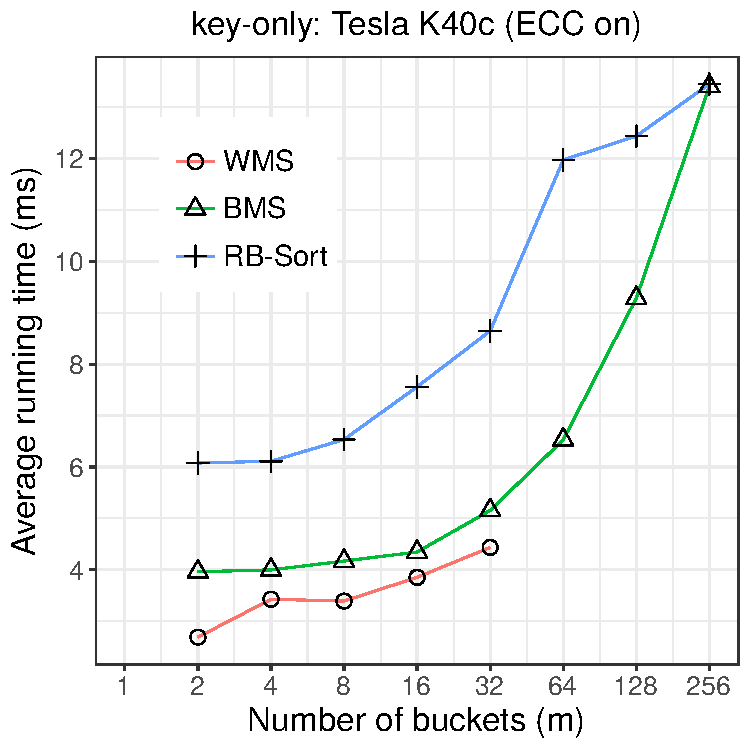
\includegraphics[width=0.32\linewidth]{avg_plot_k_k40_on.pdf}
}
\subfloat[Key-only: K40c (ECC off)]{
        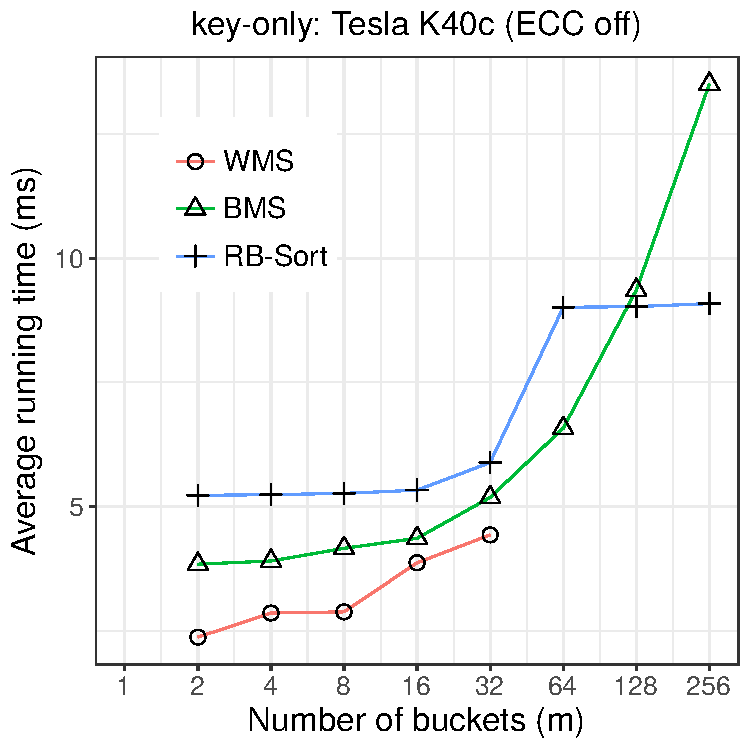
\includegraphics[width=0.32\linewidth]{avg_plot_k_k40_off.pdf}
}
\subfloat[Key-only: GTX 1080]{
        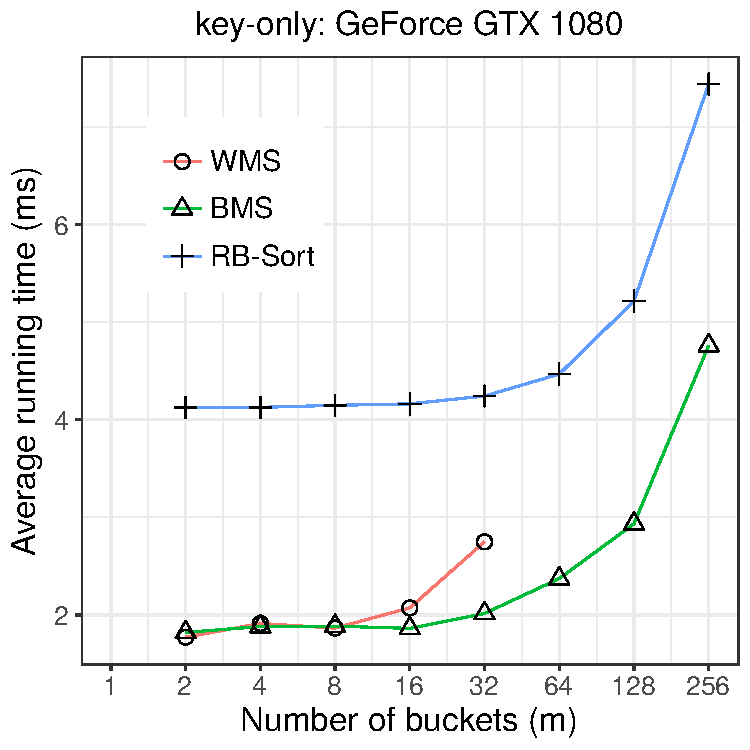
\includegraphics[width=0.32\linewidth]{avg_plot_k_gtx.pdf}
}\\
\subfloat[Key-value: K40c (ECC on)]{
        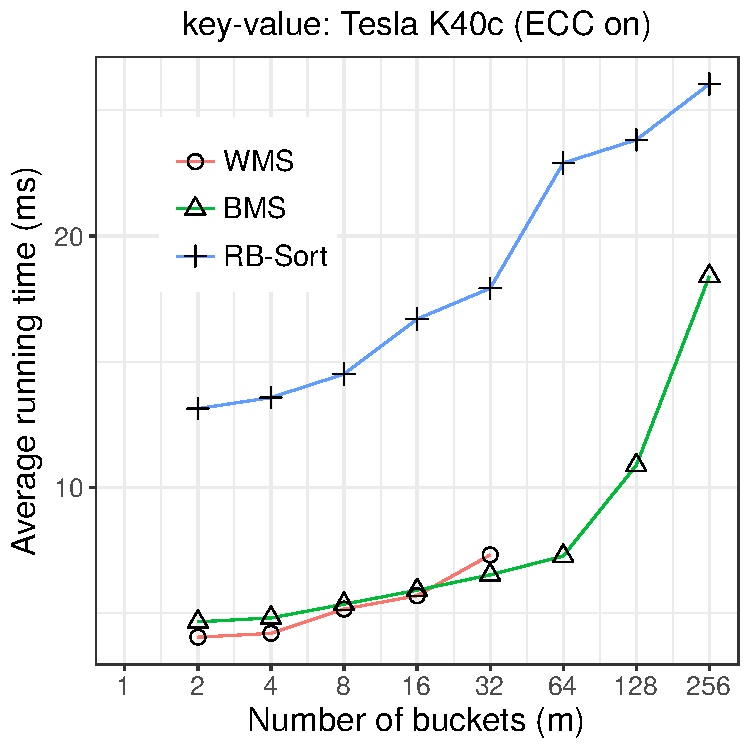
\includegraphics[width=0.32\linewidth]{avg_plot_kv_k40_on.pdf}
}
\subfloat[Key-value: K40c (ECC off)]{
        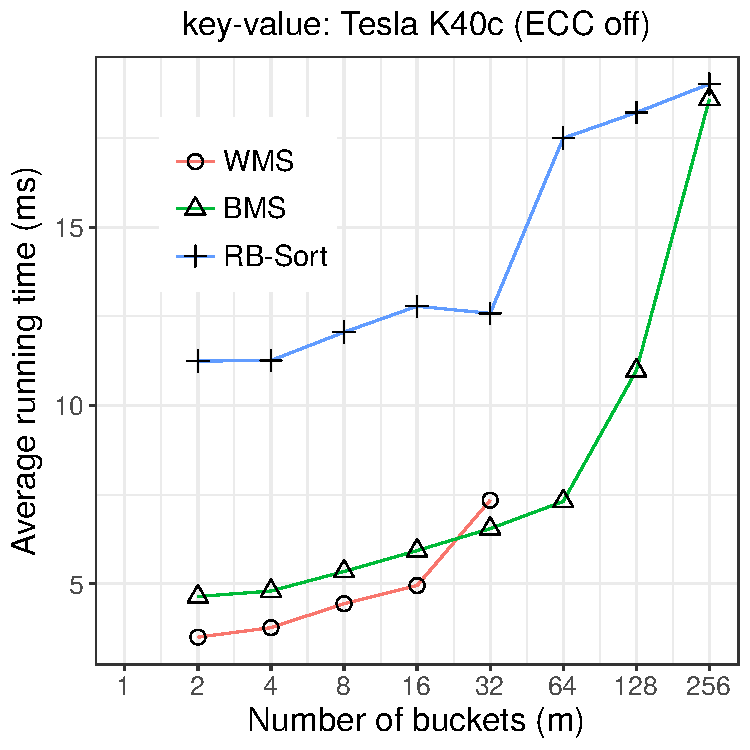
\includegraphics[width=0.32\linewidth]{avg_plot_kv_k40_off.pdf}
}
\subfloat[Key-value: GTX 1080]{
        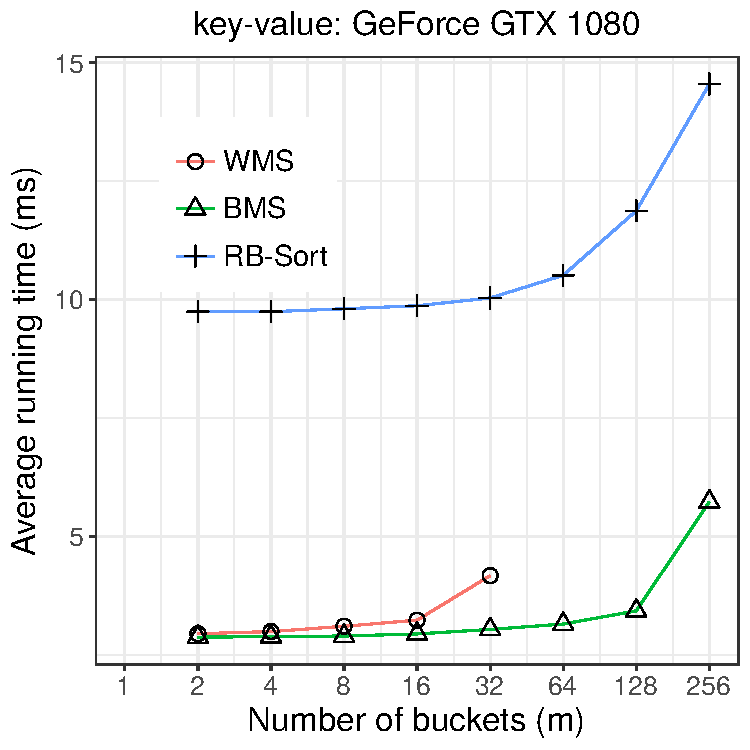
\includegraphics[width=0.32\linewidth]{avg_plot_kv_gtx.pdf}
}
\caption{Average running time (ms) versus number of buckets for all multisplit methods: (a,b,c) key-only, 32~M elements (d,e,f) key-value, 32~M elements.} \label{fig:avg_time}
\end{figure}

Figure~\ref{fig:avg_time} shows the average running time of our multisplit algorithms versus the number of buckets ($m$).
For small $m$, BMS has the best locality (at the cost of substantial local work), but WMS achieves fairly good locality coupled with simple local computation; it is the fastest choice for small $m$ ($\leq 32$ [key-only, Tesla K40c], $\leq 16$ [key-value, Tesla K40c], and $\leq2$ [key-only, GeForce GTX 1080]).
For larger $m$, the superior memory locality of BMS coupled with a minimized global scan cost makes it the best method overall.

Our multisplit methods are also almost always superior to the RB-sort method (except for the $m \geq 128$ key-only case on Tesla K40c with ECC off).
This is partly because of the extra overheads that we introduced for bucket identification and creating the label vector, and packing/unpacking stages for key-value multisplit.
Even if we ignore these overheads, since RB-sort performs its operations and permutations over the label vector as well as original key (key-value) elements, its data movements are more expensive compared to all our multisplit methods that instead only process and permute original key (key-value) elements.\footnote{In our comparisons against our own multisplit methods, RB-sort will be the best sort-based multisplit method as long as our bucket identifier cannot be interpreted as a selection of some consecutive bits in its key's binary representation (i.e., $\defn{f}(u) = (u \gg k) \& (2^{r}-1)$ for some $k$ and $r$). Otherwise, these cases can be handled directly by a radix sort over a selection of bits (from the $k$-th bit until the $(k+r)$-th bit) and do not require the extra overhead that we incur in RB-sort (i.e., sorting certain bits from input keys is equivalent to a stable multisplit solution). We will discuss this more thoroughly in Section~\ref{subsec:multisplit_sort}.}

For our user-defined delta-buckets and with a uniform distribution of keys among all 32-bit integers, by comparing Table~\ref{table:reference}~and~Table~\ref{table:timing} it becomes clear that our multisplit method outperforms radix sort by a significant margin. Figure~\ref{fig:speedup} shows our achieved speedup against the regular 32-bit radix sort performance (Table~\ref{table:reference}).
We can achieve up to 9.7x (and 10.8x) for key-only (and key-value) multisplits against radix sort.

\begin{figure}
\centering
\subfloat[Key-only: K40c (ECC on)]{
        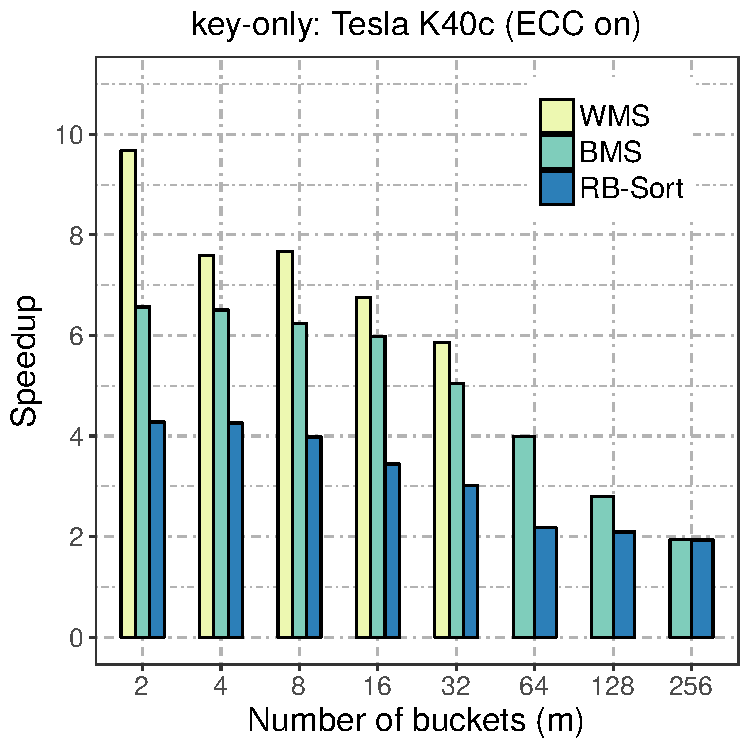
\includegraphics[width=0.32\linewidth]{speedup_k_k40_on.pdf}
}
\subfloat[Key-only: K40c (ECC off)]{
        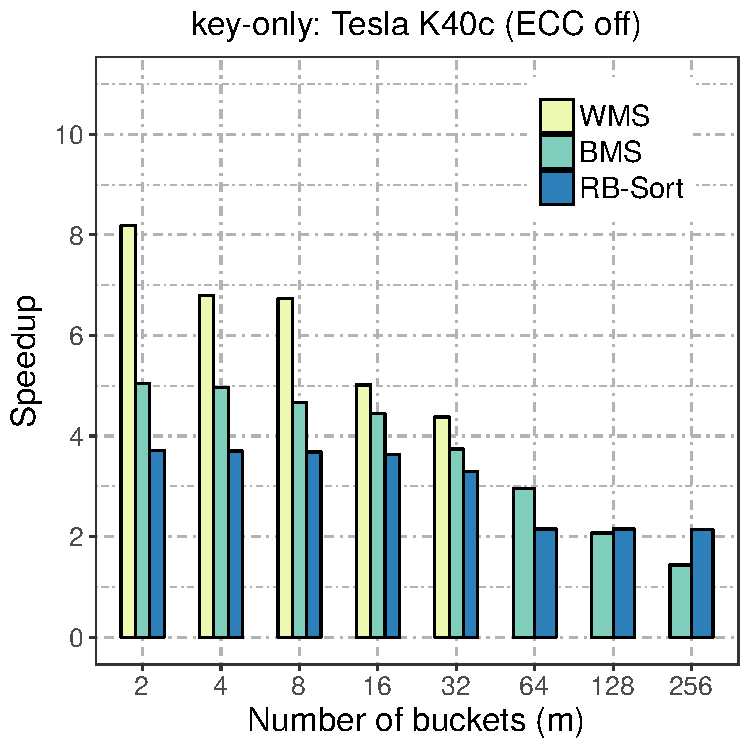
\includegraphics[width=0.32\linewidth]{speedup_k_k40_off.pdf}
}
\subfloat[Key-only: GTX 1080]{
        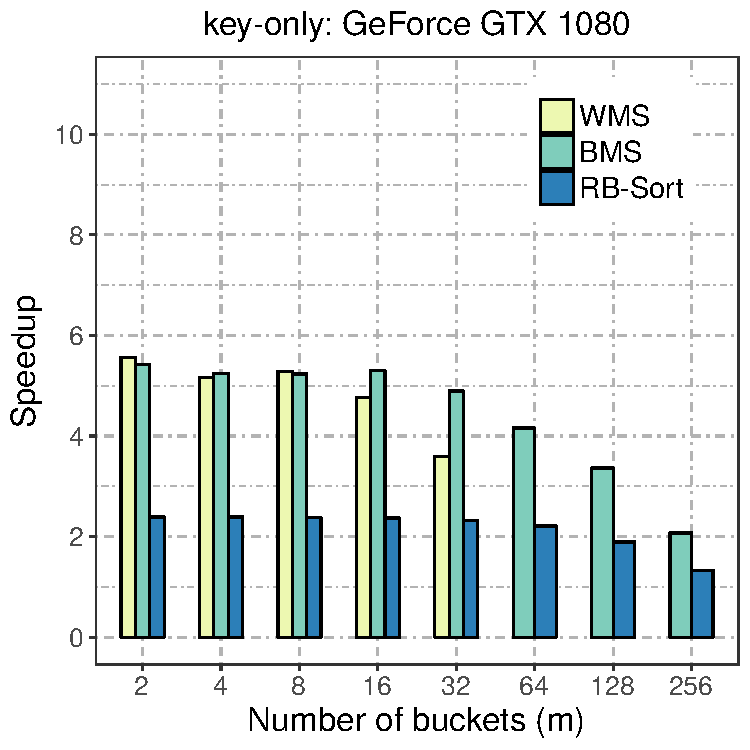
\includegraphics[width=0.32\linewidth]{speedup_k_gtx.pdf}
}\\
\subfloat[Key-value: K40c (ECC on)]{
        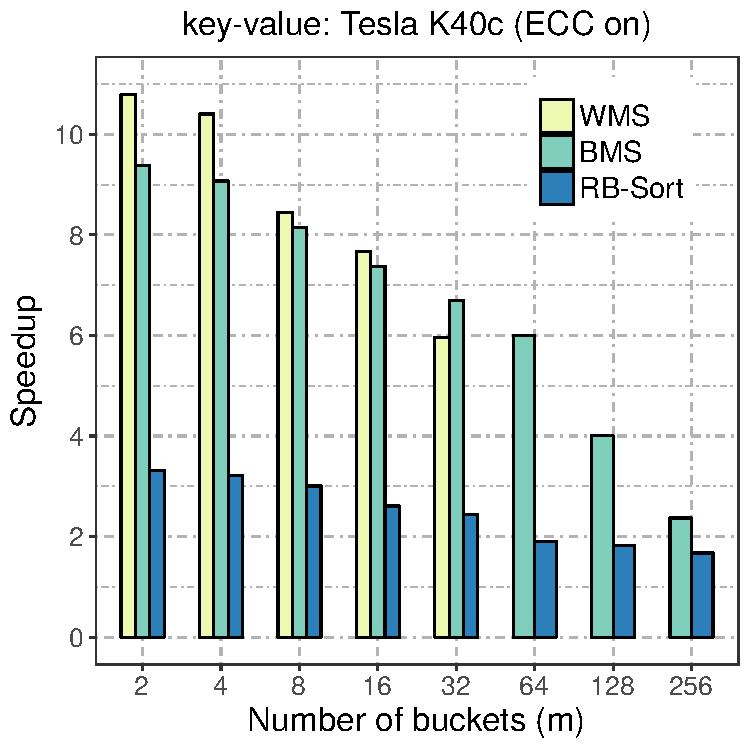
\includegraphics[width=0.32\linewidth]{speedup_kv_k40_on.pdf}
}
\subfloat[Key-value: K40c (ECC off)]{
        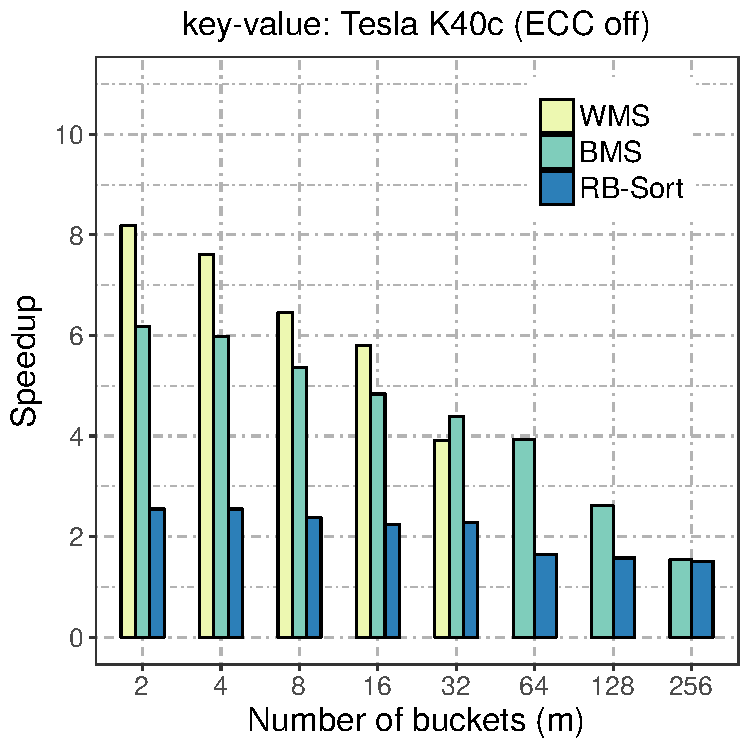
\includegraphics[width=0.32\linewidth]{speedup_kv_k40_off.pdf}
}
\subfloat[Key-value: GTX 1080]{
        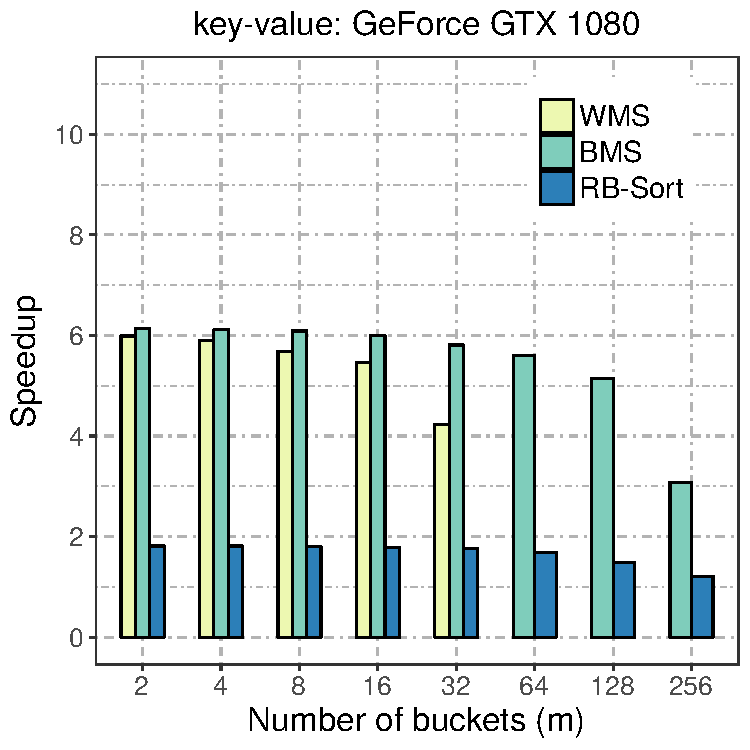
\includegraphics[width=0.32\linewidth]{speedup_kv_gtx.pdf}
}
\caption{Achieved speedup against regular radix sort versus number of buckets for all multisplit methods: (a,b,c) key-only, (d,e,f) key-value. Both scenarios are over 32~M elements random elements uniformly distributed among buckets, and delta-bucket identifiers.} \label{fig:speedup}
\end{figure}

\subsubsection{Processing rate, and multisplit speed of light}\label{sec:perf_rate}
It is instructive to compare any implementation to its ``speed of light'': a processing rate that could not be exceeded.
For multisplit's speed of light, we consider that computations take no time and all memory accesses are fully coalesced. Our parallel model requires one single global read of all elements before our global scan operation to compute histograms. We assume the global scan operation is free. Then after the scan operation, we must read all keys (or key-value pairs) and then store them into their final positions. For multisplit on keys, we thus require 3 global memory accesses per key; 5 for key-value pairs.
Our Tesla K40c has a peak memory bandwidth of 288~GB/s, so the speed of light for keys, given the many favorable assumptions we have made for it, is 24~Gkeys/s, and for key-value pairs is 14.4~G~pairs/s.
Similarly, our GTX 1080 has 320~GB/s memory bandwidth and similar computations give us a speed of light of 26.6 G~keys/s for key-only case and 16~Gpairs/s for key-value pairs.

Table~\ref{table:ms_rate} shows our processing rates for 32M keys and key-value pairs using delta-buckets and with keys uniformly distributed among all buckets.
WMS has the highest peak throughput (on 2 buckets): 12.48~Gkeys/s on Tesla K40c (ECC on), 14.15~Gkeys/s on Tesla K40c (ECC off), and 18.93~Gkeys/s on GeForce GTX 1080.
We achieve more than half the speed of light performance (60\% on Tesla K40c and 71\% on GeForce GTX 1080) with 2 buckets.
As the number of buckets increases, it is increasingly more costly to sweep all input keys to compute final permutations for each element.
We neglected this important part in our speed of light estimation.
With 32 buckets, we reach 7.57 G~keys/s on Tesla K40c and 16.64 G~keys/s on GeForce GTX 1080. While this is less than the 2-bucket case, it is still a significant fraction of our speed of light estimation (32\% and 63\% respectively).

The main obstacles in achieving the speed of light performance are 1)~non-coalesced memory writes and 2)~the non-negligible cost that we have to pay to sweep through all elements and compute permutations.
The more registers and shared memory that we have (fast local storage as opposed to the global memory), the easier it is to break the whole problem into larger subproblems and localize required computations as much as possible. This is particularly clear from our results on the GeForce GTX 1080 compared to the Tesla K40c, where our performance improvement is proportionally more than just the GTX 1080's global memory bandwidth improvement (presumably because of more available shared memory per SM).
% \john{Then say why! Is it more registers, faster registers, more shared memory, faster shared memory?}
% Our achieved rates significantly outperform regular 32-bit radix sort (Table~\ref{table:reference}).
\begin{table}
\centering
\tiny
\resizebox{\columnwidth}{!}{
\begin{tabular}{lll cccccccc}
\toprule
& & & \multicolumn{8}{c}{Throughput (speedup against radix-sort)} \\
\cmidrule{4-11}
& & & \multicolumn{8}{c}{Number of buckets (m)} \\
\cmidrule{4-11}
& & Method  & 2 & 4 & 8 & 16 & 32 & 64 & 128 & 256 \\
\midrule
    \multirow{8}{*}{\begin{turn}{90}K40c (ECC on)\end{turn}}
    & \multirow{4}{*}{\begin{turn}{90}\tiny key-only\end{turn}}
    & DMS
        & 8.79 (6.8 x) &  8.36 (6.5 x) &  6.91 (5.4 x) &  6.90 (5.4 x) &  3.26 (2.5 x) & -- & -- & -- \\ 
    & & WMS 
        & \textbf{12.48 (9.7 x)} &  \textbf{9.79 (7.6 x)} &  \textbf{9.90 (7.7 x)} &  \textbf{8.71 (6.8 x)} &  \textbf{7.57 (5.9 x)} & -- & -- & -- \\ 
    & & BMS
        & 8.47 (6.6 x) &  8.39 (6.5 x) &  8.05 (6.2 x) &  7.72 (6.0 x) &  6.51 (5.0 x) &  \textbf{5.14 (4.0 x)} &  \textbf{3.61 (2.8 x)} &  \textbf{2.50 (1.9 x)} \\
    & & RB-sort  
        & 5.52 (4.3 x) &  5.49 (4.3 x) &  5.14 (4.0 x) &  4.44 (3.4 x) &  3.88 (3.0 x) &  2.80 (2.2 x) &  2.70 (2.1 x) &  2.50 (1.9 x) \\
\cmidrule{2-11}
    & \multirow{4}{*}{\begin{turn}{90}\tiny key-value\end{turn}} 
    & DMS
        & 6.90 (9.0 x) &  6.31 (8.2 x) &  5.62 (7.3 x) &  5.62 (7.3 x) &  1.94 (2.5 x) & -- & -- & -- \\
    & & WMS 
        & \textbf{8.31 (10.8 x)} &  \textbf{8.01 (10.4 x)} &  \textbf{6.51 (8.5 x)} &  \textbf{5.90 (7.7 x)} &  4.59 (6.0 x) & -- & -- & -- \\ 
    & & BMS
        & 7.22 (9.4 x) &  6.98 (9.1 x) &  6.27 (8.1 x) &  5.68 (7.4 x) &  \textbf{5.15 (6.7 x)} &  \textbf{4.62 (6.0 x)} &  \textbf{3.09 (4.0 x)} &  \textbf{1.82 (2.4 x)} \\ 
    & & RB-sort  
        & 2.56 (3.3 x) &  2.47 (3.2 x) &  2.31 (3.0 x) &  2.01 (2.6 x) &  1.87 (2.4 x) &  1.47 (1.9 x) &  1.41 (1.8 x) &  1.29 (1.7 x) \\  
\midrule
\midrule
    \multirow{8}{*}{\begin{turn}{90}K40c (ECC off)\end{turn}}
    & \multirow{4}{*}{\begin{turn}{90}\tiny key-only\end{turn}} 
    & DMS
        & 8.99 (5.2 x) &  8.52 (4.9 x) &  6.98 (4.0 x) &  4.94 (2.9 x) &  3.26 (1.9 x) & -- & -- & -- \\
    & & WMS 
        & \textbf{14.15 (8.2 x)} &  \textbf{11.74 (6.8 x)} &  \textbf{11.65 (6.7 x)} &  \textbf{8.68 (5.0 x)} &  \textbf{7.57 (4.4 x)} & -- & -- & -- \\ 
    & & BMS
        & 8.74 (5.1 x) &  8.59 (5.0 x) &  8.07 (4.7 x) &  7.69 (4.4 x) &  6.47 (3.7 x) &  \textbf{5.10 (2.9 x)} &  3.59 (2.1 x) &  2.48 (1.4 x)  \\ 
    & & RB-sort
        & 6.42 (3.7 x) &  6.40 (3.7 x) &  6.37 (3.7 x) &  6.30 (3.6 x) &  5.70 (3.3 x) &  3.72 (2.2 x) &  \textbf{3.72 (2.1 x)} &  \textbf{3.69 (2.1 x)} \\ 
\cmidrule{2-11}
    & \multirow{4}{*}{\begin{turn}{90}\tiny key-value\end{turn}} 
    & DMS 
        & 8.99 (7.7 x) &  7.05 (6.0 x) &  5.71 (4.9 x) &  3.98 (3.4 x) &  1.96 (1.7 x) & -- & -- & -- \\
    & & WMS 
        & \textbf{9.58 (8.2 x)} &  \textbf{8.90 (7.6 x)} &  \textbf{7.55 (6.5 x)} &  \textbf{6.78 (5.8 x)} &  4.57 (3.9 x) & -- & -- & -- \\ 
    & & BMS
        & 7.23 (6.2 x) &  6.99 (6.0 x) &  6.28 (5.4 x) &  5.66 (4.8 x) &  \textbf{5.13 (4.4 x)} &  \textbf{4.59 (3.9 x)} &  \textbf{3.06 (2.6 x)} &  \textbf{1.81 (1.5 x)} \\ 
    & & RB-sort
        & 2.98 (2.6 x) &  2.98 (2.5 x) &  2.78 (2.4 x) &  2.63 (2.2 x) &  2.67 (2.3 x) &  1.92 (1.6 x) &  1.84 (1.6 x) &  1.76 (1.5 x) \\  
\midrule
\midrule
    \multirow{8}{*}{\begin{turn}{90}GTX 1080  \end{turn}}
    & \multirow{4}{*}{\begin{turn}{90}\tiny key-only\end{turn}} 
    & DMS
    & 17.67 (5.2 x) &  14.38 (4.2 x) &  11.00 (3.2 x) &  7.73 (2.3 x) &  5.54 (1.6 x) & -- & -- & -- \\
    & & WMS 
        & \textbf{18.93 (5.6 x)} &  17.54 (5.2 x) &  \textbf{17.98 (5.3 x)} &  16.18 (4.8 x) &  12.20 (3.6 x) & -- & -- & -- \\ 
    & & BMS
        & 18.42 (5.4 x) &  \textbf{17.84 (5.2 x)} &  17.79 (5.2 x) &  \textbf{18.01 (5.3 x)} &  \textbf{16.64 (4.9 x)} &  \textbf{14.14 (4.2 x)} &  \textbf{11.43 (3.4 x)} &  \textbf{7.05 (2.1 x)} \\ 
    & & RB-sort
        & 8.13 (2.4 x) &  8.13 (2.4 x) &  8.09 (2.4 x) &  8.06 (2.4 x) &  7.91 (2.3 x) &  7.51 (2.2 x) &  6.43 (1.9 x) &  4.51 (1.3 x) \\ 
\cmidrule{2-11}
    & \multirow{4}{*}{\begin{turn}{90}\tiny key-value\end{turn}} 
    & DMS
        & 11.17 (5.9 x) &  9.75 (5.1 x) &  7.07 (3.7 x) &  4.95 (2.6 x) &  3.51 (1.8 x) & -- & -- & -- \\
    & & WMS 
        & 11.38 (6.0 x) &  11.21 (5.9 x) &  10.81 (5.7 x) &  10.37 (5.5 x) &  8.04 (4.2 x) & -- & -- & -- \\ 
    & & BMS
        & \textbf{11.67 (6.1 x)} &  \textbf{11.62 (6.1 x)} &  \textbf{11.57 (6.1 x)} &  \textbf{11.40 (6.0 x)} &  \textbf{11.04 (5.8 x)} &  \textbf{10.64 (5.6 x)} &  \textbf{9.78 (5.1 x)} &  \textbf{5.85 (3.1 x)}  \\ 
    & & RB-sort
        & 3.44 (1.8 x) &  3.44 (1.8 x) &  3.42 (1.8 x) &  3.40 (1.8 x) &  3.34 (1.8 x) &  3.19 (1.7 x) &  2.83 (1.5 x) &  2.31 (1.2 x) \\  

\bottomrule
\end{tabular}
}
  \caption{Multisplit with delta-buckets and $2^{25}$ random keys uniformly distributed among $m$ buckets. Achieved processing rates (throughput) are shown in Gkeys/s (or Gpairs/s for key-value pairs). In parenthesis speedup against regular CUB's radix-sort over input elements are shown. }\label{table:ms_rate}
\end{table}

%%%%%%%%%%%%%%%%%%%%%%%%%%%%%%%%%%%%%%%%%%%%%%%%%%%%%%%%%%%%%
\subsubsection{Performance on different GPU microarchitectures}\label{subsec:perf_architecture}
In our design we have not used any (micro)architecture-dependent optimizations and hence we do not expect radically different behavior on different GPUs, other than possible speedup differences based on the device's capability.
Here, we briefly discuss some of the issues related to hardware differences that we observed in our experiments.

\paragraph{Tesla K40c} It is not yet fully disclosed whether disabling ECC (which is a hardware feature and requires reboot after modifications) has any direct impact besides available memory bandwidth (such as available registers, etc.).
% \saman{will spend a few hours by the profiler to investigate more}
For a very small number of buckets, our local computations are relatively cheap and hence having more available bandwidth (ECC off compared to ECC on) results in better overall performance (Table~\ref{table:ms_rate}).
The performance gap, however, decreases as the number of buckets increases.
This is mainly because of computational bounds due to the increase in ballot, shuffle, and numerical integer operations as $m$ grows.
% This is mainly because we are also getting more compute bounded (by having to deal with more ballots, shuffles and numerical integer computations per read input element, as $m$ grows).
% \saman{one part that I still am not sure about, is that I'm getting marginally better results for my key-only with ECC on compared to ECC off. I will do more profiling to see if I can say something useful here.}

CUB's radix sort greatly improves on Tesla K40c when ECC is disabled (Table~\ref{table:reference}), and because of it, RB-sort improves accordingly.
CUB has particular architecture-based fine-grained optimizations, and we suspect it is originally optimized for when ECC is disabled to use all hardware resources to exploit all available bandwidth as much as possible. We will discuss CUB further in Section~\ref{subsec:multisplit_sort}.
RB-sort's speedups in Fig.~\ref{fig:speedup} are relatively less for when ECC is disabled compared to when it is enabled. The reason is not because RB-sort performs worse (Table~\ref{table:ms_rate} shows otherwise), but rather because  CUB's regular radix sort (that we both use in RB-sort and compare against for speedup computations) improves when ECC is disabled (Table~\ref{table:reference}).

\paragraph{GeForce GTX 1080}
This GPU is based on NVIDIA's latest ``Pascal'' architecture. It both increases global memory bandwidth (320~GB/s) and appears to be better at hiding memory latency caused by non-coalesced memory accesses. The GTX 1080 also has more available shared memory per SM, which results in more resident thread-blocks within each SM.
As a result, it is much easier to fully occupy the device, and our results (Table~\ref{table:ms_rate}) show this.
%%%%%%%%%%%%%%%%%%%%%%%%%%%%%%%%%%%%%%%%%%%%%%%%%%%%%%%%%%%%%
\subsection{Performance for more than 256 buckets}\label{subsec:perf_more}
So far, we have only characterized problems with $m \leq 256$ buckets.
As we noted in Section~\ref{sec:radix}, we expect that as the number of buckets increases, multisplit converges to a sorting problem and we should see the performance of our multisplits and sorting-based multisplits converge as well.

The main obstacle for efficient implementation of our multisplits for large  bucket counts is the limited amount of shared memory available on GPUs for each thread-block.
Our methods rely on having privatized portions of shared memory with $m$ integers per warp (total of $32m$ bits/warp).
As a result, as $m$ increases, we require more shared storage, which limits the number of resident thread-blocks per SM, which limits our ability to hide memory latency and hurts our performance.
Even if occupancy was not the main issue, with the current GPU shared memory sizes (48~KB per SM for Tesla K40c, and 96~KB per SM to be shared by two blocks on GeForce GTX 1080), it would only be physically possible for us to scale our multisplit up to about $m = 12\text{k}/{N_\text{warp}}$ (at most 12k buckets if we use only one warp per thread-block).

In contrast, RB-sort does not face this problem. Its labeling stage (and the packing/unpacking stage required for key-value pairs) are independent of the number of buckets. However, the radix sort used for RB-sort's sorting stage is itself internally scaled by a factor of $\log m$, which results in an overall logarithmic dependency for RB-sort vs.\ the number of buckets.

\paragraph{Solutions for larger multisplits ($m>256$)}
Our solution for handling more buckets is similar to how radix sort handles the same scalability problem: iterative usage of multisplit over $m' \leq 256$ buckets. However, this is not a general solution and it may not be possible for any general bucket identifier.
For example, for delta-buckets with 257 buckets, we can treat the first 2 buckets together as one single super-bucket which makes the whole problem into 256 buckets. Then, by two rounds of multisplit 1)~on our new 256 buckets, 2)~on the initial first 2 buckets (the super-bucket), we can have a stable multisplit result.
This approach can potentially be extended to any number of buckets, but only if our bucket identifier is suitable for such modifications.
There are some hypothetical cases for which this approach is not possible (for instance, if our bucket identifier is a random hash function, nearby keys do not necessarily end up in nearby buckets).

Nevertheless, if iterative usage is not possible, it is best to use RB-sort instead, as it appears to be quite competitive for a very large number of buckets. As a comparison with regular radix sort performance, on Tesla K40c (ECC on), RB-sort outperforms radix sort up to almost 32k keys and 16k key-value pairs. However, we reiterate that unlike RB-sort, which is always a correct solution for multisplit problems, direct usage of radix sort is not always a possible solution.

%%%%%%%%%%%%%%%%%%%%%%%%%%%%%%%%%%%%%%%%%%%%%%%%%%%%%%%%%%%%%
\subsection{Initial key distribution over buckets}\label{subsec:perf_distribution}
So far we have only considered scenarios in which initial key elements were uniformly distributed over buckets (i.e., a uniform histogram).
In our implementations we have considered small subproblems (warp-sized for WMS and block-sized for BMS) compared to the total size of our initial key vector.
Since these subproblems are relatively small, having a non-uniform distribution of keys means that we are more likely to see empty buckets in some of our subproblems; in practice, our methods would behave as if there were fewer buckets for those subproblems.
All of our \emph{computations} (e.g., warp-level histograms) are data-independent and, given a fixed bucket count, would have the same performance for any distribution. However, our \emph{data movement}, especially after reordering, would benefit from having more elements within fewer buckets and none for some others (resulting in better locality for coalesced global writes). Consequently, the uniform distribution is the worst-case scenario for our methods.

As an example of a non-uniform distribution, consider the binomial distribution.
In general $B(m-1,p)$ denotes a binomial distribution over $m$ buckets with a probability of success $p$. For example, the probability that a key element belongs to bucket $0\leq k < m$ is $\binom{m-1}{k}p^k {(1-p)}^{m-k-1}$.
This distribution forces an unbalanced histogram as opposed to the uniform distribution.
Note that by choosing $p=0.5$, the expected number of keys within the $k$th bucket will be $n\binom{m-1}{k} 2^{1-m}$.
For example, with $n=2^{25}$ elements and $m=256$ total buckets, there will be on average almost 184 empty buckets (72\%).
Such an extreme distribution helps us evaluate the sensitivity of our multisplit algorithms to changes in input distribution.

Figure~\ref{fig:binomial} shows the average running time versus the number of buckets for BMS and RB-sort with binomial and uniform distributions, on our Tesla K40c (ECC off).
There are two immediate observations here.
First, as the number of buckets increases, both algorithms become more sensitive to the input distribution of keys.
This is mainly because, on average, there will be more empty buckets and our data movement will resemble situations where there are essentially much fewer number of buckets than the actual $m$.
Second, the sensitivity of our algorithms increases in key-value scenarios when compared to key-only scenarios, mainly because data movement is more expensive in the latter. As a result, any improvement in our data movement patterns (here caused by the input distribution of keys) in a key-only multisplit will be almost doubled in a key-value multisplit.

\begin{figure}
  \centering
  \subfloat[Key-only]
  {
    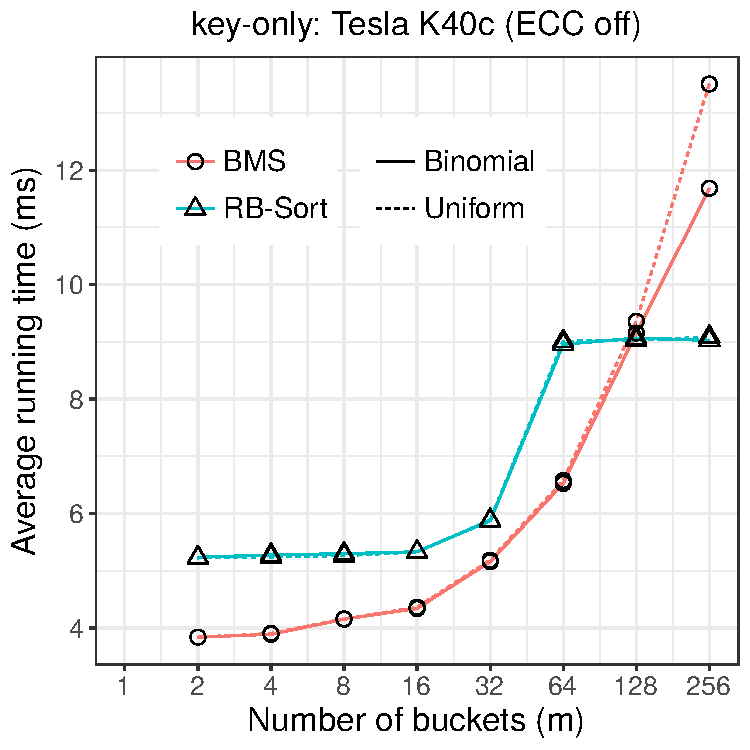
\includegraphics[width = 0.4\linewidth]{avg_dist_k_k40_off.pdf}
    \label{fig:dist_k}
  }
  \subfloat[Key-value]
  {
    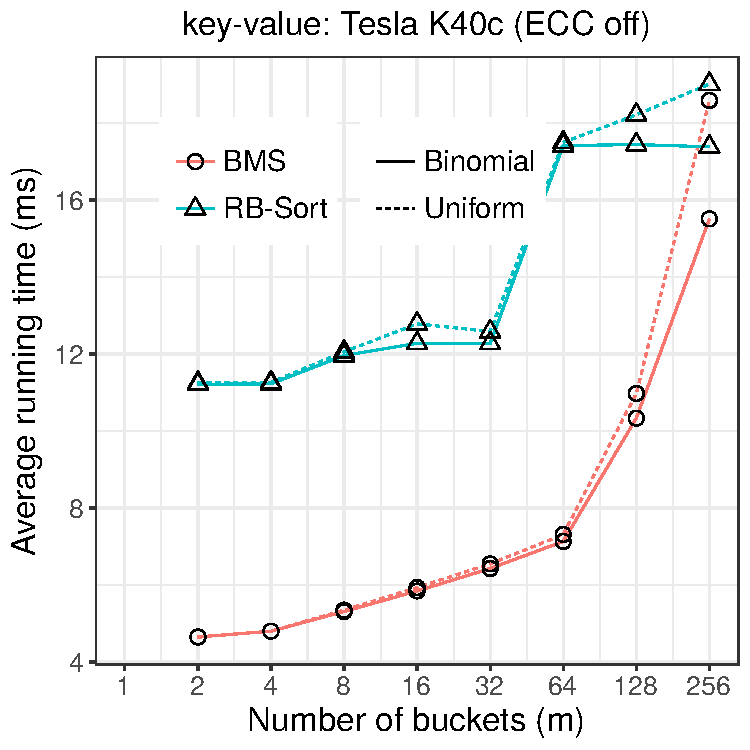
\includegraphics[width = 0.4\linewidth]{avg_dist_kv_k40_off.pdf}
    \label{fig:dist_kv}
  }
  \caption{Average running time (ms) vs.\ number of buckets ($m$) for two different initial key distributions: (a) a uniform distribution and (b) the binomial distribution $B(m-1,0.5)$.}\label{fig:binomial}
\end{figure}

To get some statistical sense over how much improvement we are getting, we ran multiple experiments with different input distributions, with delta-buckets as our bucket identifiers, and on different GPUs. Table~\ref{table:distribution} summarizes our results with $m=256$ buckets.
In this table, we also consider a milder distribution where $\alpha n$ of total keys are uniformly distributed among buckets and the rest are within one random bucket ($\alpha$-uniform).
BMS achieves up to 1.24x faster performance on GeForce GTX 1080 when input keys are distributed over buckets in the binomial distribution. Similarly, RB-sort achieve up to 1.15x faster on Tesla K40c (ECC off) with the binomial distribution.
In general, compared to our methods, RB-sort seems to be less sensitive to changes to the input distribution.

% Figure~\ref{fig:binomial} shows the average running time of BMS and RB-sort with different distributions. Both methods perform better as keys become less uniformly distributed, because on average there is less intermediate data movement. The RB-sort is more sensitive, because the internal hierarchical approach in radix sort helps it to put most of its effort on more common bits.
% With a uniform distribution, all bits are equally populated, so all bits get the same attention. \john{There's no real conclusion in this paragraph. I want the text to say something like ``our methods look correspondingly \{better, worse\} than RB-sort as the distribution diverges from uniform''.}

\begin{table}
\centering
\scriptsize
% \resizebox{\columnwidth}{!}{
\begin{tabular}{lll cc | cc | cc}
\toprule
Type & Method & Distribution & \multicolumn{2}{c}{Tesla K40c (ECC on)} & \multicolumn{2}{c}{Tesla K40c (ECC off)} & \multicolumn{2}{c}{GeForce GTX 1080} \\
\midrule
    \multirow{6}{*}{\begin{turn}{90}Key-only\end{turn}}
    & \multirow{3}{*}{BMS}
    & Uniform
        % &  2503.578 & 2484.341 & 7045.623  \\
        &  2.50 &  & 2.48 &  & 7.05 &   \\
    & & 0.25-uniform
        % &   2641.196 & 2608.820 & 7363.078   \\
        &   2.64 & 1.06x & 2.61 & 1.05x & 7.36  & 1.05x    \\
    & & Binomial
        % &   2886.794 & 2871.922 & 7890.201   \\
        &   2.89 & 1.15x & 2.87  & 1.16x & 7.89 & 1.11x    \\
\cmidrule{2-9}
    & \multirow{3}{*}{RB-sort}
    & Uniform
        % &  2495.076 & 3692.785 & 4508.853  \\
        &  2.50 &  & 3.69 &  & 4.51 &   \\
    & & 0.25-uniform
        % &  2690.844 & 3706.512 & 4558.114  \\
        &  2.69  & 1.08x  & 3.71  & 1.00x  & 4.56  & 1.01x   \\
    & & Binomial
        % &   2801.709 & 3717.827 & 4947.911   \\
        &   2.80  & 1.12x  & 3.72  & 1.01x  & 4.95  & 1.10x    \\
\cmidrule{1-9}
\cmidrule{1-9}
\multirow{6}{*}{\begin{turn}{90}Key-value\end{turn}}
    & \multirow{3}{*}{BMS}
    & Uniform
        % &  1823.524 & 1805.371 & 5852.571  \\
        &  1.82 &  & 1.81 &  & 5.85 &   \\
    & & 0.25-uniform
        % &   1990.875 & 1995.536 & 6706.594   \\
        &   1.99  & 1.10x & 2.00  & 1.11x  & 6.71  & 1.15x    \\
    & & Binomial
        % &   2182.210 & 2163.570 & 7284.155   \\
        &   2.18  & 1.20x  & 2.16  & 1.20x  & 7.28 & 1.24x    \\
\cmidrule{2-9}
    & \multirow{3}{*}{RB-sort}
    & Uniform
        % &  1288.269 & 1764.892 & 2305.981  \\
        & 1.29 & & 1.77 &  & 2.31 &   \\
    & & 0.25-uniform
        % &  1453.948 & 1807.510 & 2331.702  \\
        &  1.45  & 1.13x  & 1.81  & 1.02x  & 2.33  & 1.01x    \\
    & & Binomial
        % &   1478.142 & 1930.571 & 2522.792   \\
        &   1.48  & 1.15x   & 1.93  & 1.9x  & 2.52  & 1.09x    \\

\bottomrule
\end{tabular}
% }
\caption{Processing rate (billion elements per second) as well as speedup against the uniform distribution for delta-bucket multisplit with different input distributions. All cases are with $m=256$ buckets.}\label{table:distribution}
\end{table}

